\documentclass[a4paper,10pt]{article}
\usepackage[utf8]{inputenc}
\usepackage[spanish]{babel}
\usepackage[affil-it]{authblk}
\usepackage{enumerate}
\usepackage{graphicx}
\usepackage{hyperref}
\usepackage{amsmath}
\usepackage{amssymb}
\usepackage{cancel}
\usepackage[usenames, dvipsnames]{color}
\usepackage{tikz}
\usepackage[labelfont=bf]{caption}
\usepackage{subcaption} %Multiple images
\usepackage{multicol} % Multiple columns
\usepackage{float}
\usepackage{cleveref}
 \usepackage{relsize} % bigger math symbols
\usepackage[margin=1.4in]{geometry}
\usepackage[titletoc,toc,title]{appendix}
\usepackage{enumitem}
\usetikzlibrary{calc}
\numberwithin{equation}{section}

\graphicspath{Tarea10/}

%Appendices in spanish
\renewcommand{\appendixname}{Ap\'endices}
\renewcommand{\appendixtocname}{Ap\'endices}
\renewcommand{\appendixpagename}{Ap\'endices}

%Zero delimiter
\newcommand{\zerodel}{.\kern-\nulldelimiterspace}

%Columns separation
\setlength{\columnsep}{1cm}

%Indentation
\setlength{\parindent}{0ex}

%Multiple References

\crefrangelabelformat{equation}{(#3#1#4--#5\crefstripprefix{#1}{#2}#6)}

\usepackage{xparse}

%Boxes

\newcommand*{\boxcolor}{blue}
\makeatletter
\renewcommand{\boxed}[1]{\textcolor{\boxcolor}{%
\tikz[baseline={([yshift=-1ex]current bounding box.center)}] \node [rectangle, minimum width=1ex,rounded corners,draw] {\normalcolor\m@th$\displaystyle#1$};}}
 \makeatother

%Constantes
\newcommand{\euler}{\mathrm{e}}
\newcommand{\im}{i}

%Lemas, teoremas, definiciones y pruebas
\newcommand{\definicion}{\textbf{Definición: }}
\newcommand{\lema}{\textbf{Lema: }}
\newcommand{\teorema}{\textbf{Teorema: }}
\newcommand{\prueba}{\textbf{Prueba: }}
\newcommand{\proposicion}{\textbf{Proposición: }}
\newcommand{\corolario}{\textbf{Corolario: }}


%opening
\title{Mecánica Clásica Tarea \# 10}
\author{Favio Vázquez\thanks{Correo: favio.vazquezp@gmail.com}}\affil{Instituto de Ciencias Nucleares. Universidad Nacional Autónoma de México.}
\date{}

\begin{document}

\makeatletter
\def\@maketitle{%
  \newpage
  \null
  \vskip 2em%
  \begin{center}%
  \let \footnote \thanks
    {\Large\bfseries \@title \par}%
    \vskip 1.5em%
    {\normalsize
      \lineskip .5em%
      \begin{tabular}[t]{c}%
        \@author
      \end{tabular}\par}%
    \vskip 1em%
    {\normalsize \@date}%
  \end{center}%
  \par
  \vskip 1.5em}
\makeatother

\maketitle

\section{Problema 1}

Utilizando la formulación hamiltoniana de la mecánica, encuentre las ecuaciones de 
movimiento de un péndulo doble de masas y longitudes iguales.

\vspace{.3cm}

\underline{Solución:} \vspace{.3cm}

En la figura de abajo se muestra un diagrama para el problema,

\begin{figure}[H]
 \center
 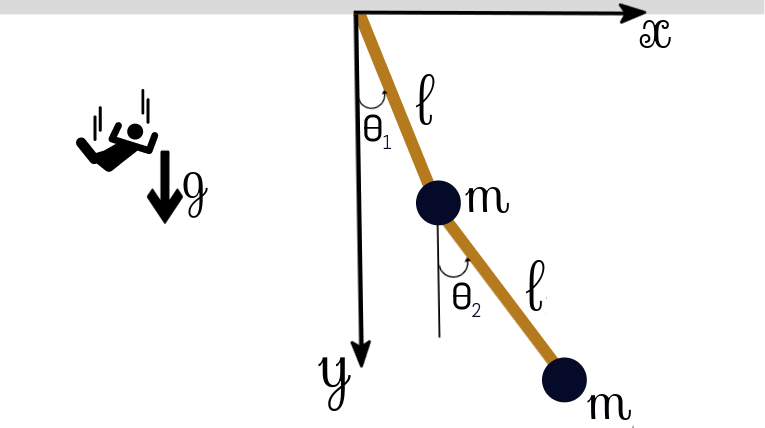
\includegraphics[scale=0.4]{problema1fig1.png}
 \caption{Péndulo doble. Como muestra el muñequito la gravedad va dirigida hacia 
 abajo.}
 \label{fig:problema1fig1}
\end{figure}

Si tomamos a $\theta_1$ y $\theta_2$ como nuestras coordenadas generalizadas, las 
coordenadas $x$ y $y$ de las dos masas serán

\begin{align}
 x_1 &= l\sen{\theta_1}, \\
 y_1 &= l\cos{\theta_1}, \\
 x_2 &= l\sen{\theta_1} + l\sen{\theta_2}, \\
 y_2 &= l\cos{\theta_1} + l\cos{\theta_2}.
\end{align}

Para construir la energía cinética del sistema necesitamos las primeras derivadas
temporales de estas ecuaciones, las cuales son

\begin{align}
 \dot{x_1} &= l\dot{\theta_1}\cos{\theta_1}, \\
 \dot{y_1} &= - l\dot{\theta_1}\sen{\theta_1}, \\
 \dot{x_2} &=  l\dot{\theta_1}\cos{\theta_1} + l\dot{\theta_2}\cos{\theta_2}, \\
 \dot{y_2} &= - l\dot{\theta_1}\sen{\theta_1} - l\dot{\theta_2}\sen{\theta_2}.
\end{align}

Entonces la energía cinética

\begin{equation}
 T = \frac{1}{2}m(\dot{x_1}^2 + \dot{y_1}^2) +  \frac{1}{2}m(\dot{x_2}^2 + \dot{y_2}^2),
\end{equation}

puede escribirse como 

\begin{align}
 T &= \frac{1}{2}m(l^2\dot{\theta_1}^2\cos^2{\theta_1} + l^2\dot{\theta_1}^2\sen^2{\theta_1} 
 + l^2\dot{\theta_1}^2\cos^2{\theta_1} + 2l^2\dot{\theta_1}\dot{\theta_2}\cos{\theta_1}\cos{\theta_2} \\
 &+ l^2\dot{\theta_2}^2\cos^2{\theta_2} + l^2\dot{\theta_1}^2\sen^2{\theta_1} + 
 2l^2\dot{\theta_1}\dot{\theta_2}\sen{\theta_1}\sen{\theta_2} + l^2\dot{\theta_2}^2\sen^2{\theta_2}),
\end{align}

\begin{equation}
 \therefore T = \frac{m}{2}l^2\left[2\dot{\theta_1}^2 + \dot{\theta_2}^2 
 + 2\dot{\theta_1}\dot{\theta_2}\cos{(\theta_1 - \theta_2)}\right]
\end{equation}

Por otra parte la energía potencial del sistema 

\begin{equation}
 V = -mgy_1 - mgy_2,
\end{equation}

puede escribirse como

\begin{equation}
 V = - mg(l\cos{\theta_1}) - mg(l\cos{\theta_1} + l\cos{\theta_2}),
\end{equation}

\begin{equation}
 \therefore V = - mgl(2\cos{\theta_1} + \cos{\theta_2}).
\end{equation}

Por lo tanto la lagrangiana del sistema es 

\begin{equation}
 L = T - V = \frac{m}{2}l^2\left[2\dot{\theta_1}^2 + \dot{\theta_2}^2 
 + 2\dot{\theta_1}\dot{\theta_2}\cos{(\theta_1 - \theta_2)}\right]
 + mgl(2\cos{\theta_1} + \cos{\theta_2}).
\end{equation}

Definimos a la hamiltoniana del sistema como

\begin{equation}
 H(q,p,t) = \sum_{k=1}^n p_k \dot{q}^k(q,p,t) - L(q,\dot{q}(q,p,t),t),
 \label{eq:hamiltonianaDoblePend}
\end{equation}

necesitamos entonces una expresión para los impulsos generalizados, y escribir a las 
velocidades generalizadas en términos de éstos. Recordamos que los impulsos generalizados 
están definidos por 

\begin{equation}
p_i = \frac{\partial L}{\partial \dot{q}^i}.
\end{equation}

En este caso tendremos dos, uno para cada coordenada generalizada

\begin{equation}
 p_{\theta_1} = \frac{\partial L}{\partial \dot{\theta_1}} = 
 2ml^2\dot{\theta_1} + ml^2\dot{\theta_2}\cos{(\theta_1 - \theta_2)},
 \label{eq:impulsoGenTheta1}
\end{equation}

\begin{equation}
 p_{\theta_2} = \frac{\partial L}{\partial \dot{\theta_2}} = 
 ml^2\dot{\theta_2} + ml^2\dot{\theta_1}\cos{(\theta_1 - \theta_2)}.
 \label{eq:impulsoGenTheta2}
\end{equation}

Ahora que tenemos expresiones para los impulsos generalizados, podemos expresar a las 
coordenadas generalizadas en función de los mismos como

\begin{equation}
 \dot{\theta_1} = \frac{\cos{(\theta_1 - \theta_2)}[- p_{\theta_1}^2 - 
 p_{\theta_2}ml^2] + p_{\theta_1}[p_{\theta_2} + ml^2\cos^2{(\theta_1 - \theta_2)}]}{m^2l^4[2 - \cos^2{(\theta_1 - \theta_2)}]}
 \label{eq:velGenTheta1}
\end{equation}

\begin{equation}
 \dot{\theta_2} = \frac{2p_{\theta_2} - 2p_{\theta_1}\cos{(\theta_1 - \theta_2)}}{ml^2[2 - \cos^2{(\theta_1 - \theta_2)}]}
 \label{eq:velGenTheta2}
\end{equation}

Usando estas ecuaciones podemos reescribir ahora la lagrangiana para que solo dependa 
de las coordenadas e impulsos generalizados, 

\begin{align*}
 L &= \frac{m}{2}l^2\left[2 \left\{ \frac{\cos{(\theta_1 - \theta_2)}[- p_{\theta_1}^2 - 
 p_{\theta_2}ml^2] + p_{\theta_1}[p_{\theta_2} + ml^2\cos^2{(\theta_1 - \theta_2)}]}{m^2l^4[2 
 - \cos^2{(\theta_1 - \theta_2)}]} \right\}^2 + \right\zerodel \\
 &2 \left\{\frac{2p_{\theta_2} - 2p_{\theta_1}\cos{(\theta_1 - 
 \theta_2)}}{ml^2[2 - \cos^2{(\theta_1 - \theta_2)}]} \right\}^2 + \\
 &2\left\{ \frac{\cos{(\theta_1 - \theta_2)}[- p_{\theta_1}^2 - 
 p_{\theta_2}ml^2] + p_{\theta_1}[p_{\theta_2} +
 ml^2\cos^2{(\theta_1 - \theta_2)}]}{m^2l^4[2 - \cos^2{(\theta_1 - \theta_2)}]}\right\}
 \left\{ \frac{2p_{\theta_2} - 2p_{\theta_1}\cos{(\theta_1 - \theta_2)}}{ml^2[2 - \cos^2{(\theta_1 - \theta_2)}]}\right\} \\
 &\left\zerodel\cos{(\theta_1 - \theta_2)}\right] + mgl(2\cos{\theta_1} + \cos{\theta_2}).
\end{align*}

Entonces la hamiltoniana del sistema puede escribirse como\footnote{El trabajo algebraico 
es largo para llegar a esta ecuación, por lo tanto solo se escribe el resultado final.}, 
utilizando las expresiones para los impulsos generalizados \eqref{eq:impulsoGenTheta1} y 
\eqref{eq:impulsoGenTheta2}, las expresiones para las velocidades generalizadas en términos 
de los impulsos generalizados \eqref{eq:velGenTheta1} y \eqref{eq:velGenTheta2}, así 
como la lagrangiana expresada sólo en términos de las coordenadas e impulsos generalizados 


\begin{equation}
 H = \frac{ml^2p_{\theta_1}^2 + 2ml^2p_{\theta_2}^2 - 
 2ml^2\cos{(\theta_1 - \theta_2)p_{\theta_1}p_{\theta_2}}}{2ml^2[2m - 
 m\cos^2{(\theta_1 - \theta_2)}]} - mgl(2\cos{\theta_1} + \cos{\theta_2}),
\end{equation}

o simplificando 

\begin{equation}
 \boxed{H = \frac{p_{\theta_1}^2 + 2p_{\theta_2}^2 - 
 2\cos{(\theta_1 - \theta_2)p_{\theta_1}p_{\theta_2}}}{4m - 
 2m\cos^2{(\theta_1 - \theta_2)}} - mgl(2\cos{\theta_1} + \cos{\theta_2})}
\end{equation}

Podemos utilizar ahora las ecuaciones de Hamilton para encontrar las ecuaciones de 
movimiento, recordamos su forma

\begin{align}
 \dot{q}^i = \frac{\partial H}{\partial p_i}, \\
 \dot{p}_i = - \frac{\partial H}{\partial q^i}.
\end{align}

Entonces las ecuaciones de movimiento, utilizando las anteriores ecuaciones serán

\begin{equation}
 \dot{\phi_1} =  \frac{\partial H}{\partial p_{\theta_1}} = 
 \frac{2p_{\theta_2} - 2p_{\theta_2}\cos{(\theta_1 - \theta_2)}}{4m - 
 2m\cos^2{(\theta_1 - \theta_2)}},
\end{equation}

\begin{equation}
 \dot{\phi_2} =  \frac{\partial H}{\partial p_{\theta_2}} = 
 \frac{4p_{\theta_2} - 2p_{\theta_1}\cos{(\theta_1 - \theta_2)}}{4m - 
 2m\cos^2{(\theta_1 - \theta_2)}},
\end{equation}

\begin{align}
\begin{split}
 \dot{p_{\theta_1}} = \frac{\partial H}{\partial \theta_1} = 
 &- \frac{4m\sen{(\theta_1 - \theta_2})\cos{(\theta_1 - \theta_2)}
 \left[p_{\theta_1}^2 - 2p_{\theta_1}p_{\theta_2}\cos{(\theta_1 - \theta_2)} + 2p_{\theta_2}^2\right]}{[4m - 2m\cos^2{(\theta_1 - \theta_2)}]^2} \\
 &+ \frac{2p_{\theta_1}p_{\theta_2}\sen{(\theta_1 - \theta_2)}}{4m - 2m\cos^2{(\theta_1 - \theta_2)}} 
 + 2mgl\sen{\theta_1},
\end{split}
\end{align}

\begin{align}
\begin{split}
 \dot{p_{\theta_2}} = \frac{\partial H}{\partial \theta_2} = 
 &\frac{4m\sen{(\theta_1 - \theta_2})\cos{(\theta_1 - \theta_2)}
 \left[p_{\theta_1}^2 - 2p_{\theta_1}p_{\theta_2}\cos{(\theta_1 - \theta_2)} + 2p_{\theta_2}^2\right]}{[4m - 2m\cos^2{(\theta_1 - \theta_2)}]^2} \\
 &- \frac{2p_{\theta_1}p_{\theta_2}\sen{(\theta_1 - \theta_2)}}{4m - 2m\cos^2{(\theta_1 - \theta_2)}} 
 + mgl\sen{\theta_2}
\end{split}
\end{align}

\section{Problema 2}

Una partícula de masa $m$ se mueve en una dimensión y la hamiltoniana del sistema 
es 

$$
H(q,p) = \frac{p^2}{2m}\euler^{-\frac{q}{a}}
$$

Encuentre las ecuaciones de movimiento y su solución. Considerando únicamente los casos 
en que $p>0$, ¿Cuál sería la fuerza que debería actuar sobre la partícula en una visión
newtoniana del este sistema? ¿Qué sentido le puede dar en este caso a las relaciones entre 
la energía total, la energía cinética y la hamiltoniana como integral de movimiento?

\vspace{.3cm}

\underline{Solución:} \vspace{.3cm}

Para encontrar las ecuaciones de movimiento utilizaremos las ecuaciones de Hamilton 
que podemos escribir, debido a que la partícula se mueve en una dimensión, como

\begin{align}
 \dot{q} = \frac{\partial H}{\partial p}, \\
 \dot{p} = - \frac{\partial H}{\partial q}.
\end{align}

Entonces tenemos que,

\begin{align}
\label{eq:2qdot1}
 \dot{q} = \frac{\cancel{2}p}{\cancel{2}m}\euler^{-\frac{q}{a}}
 = \frac{p}{m}\euler^{-\frac{q}{a}}, \\
\label{eq:2pdot1}
 \dot{p} = - \left(- \frac{1}{a}\frac{p^2}{2m}\euler^{-\frac{q}{a}}\right)
 = \frac{p^2}{2ma}\euler^{-\frac{q}{a}}.
\end{align}

Para hallar $q(t)$ nos podemos ayudar calculando $\ddot{q}$, utilizando 
\eqref{eq:2qdot1} y \eqref{eq:2pdot1}, y el hecho de que\footnote{Claramente en este caso $p>0$.}
$p^2 = \dot{q}^2m^2\euler^{\frac{2q}{a}}$,

\begin{align*}
 \ddot{q} &= \frac{\dot{p}}{m}\euler^{-\frac{q}{a}} - \frac{p\dot{q}}{ma}\euler^{-\frac{q}{a}}, \\
	  &= \euler^{-\frac{q}{a}}\left(\frac{\dot{p}}{m} - \frac{p\dot{q}}{ma}\right), \\
	  &= \euler^{-\frac{q}{a}}\left(\frac{p^2}{2m^2a}\euler^{-\frac{q}{a}} - 
	  \frac{p^2}{m^2a}\euler^{-\frac{q}{a}}\right), \\
	  &= - \euler^{-\frac{2q}{a}}\left(\frac{p^2}{2m^2a}\right), \\
	  &= - \frac{\cancel{\euler^{-\frac{2q}{a}}}}{2\cancel{m^2}a}\dot{q}^2\cancel{m^2}\cancel{\euler^{\frac{2q}{a}}},
\end{align*}

\begin{equation}
 \therefore \ddot{q} = - \frac{\dot{q}^2}{2a}
\end{equation}

Esta ecuación puede escribirse como

\begin{equation}
 m\ddot{q} = - m\frac{\dot{q}^2}{2a},
\end{equation}

donde vemos entonces que en una visión newtoniana del sistema y para el caso en que 
$p > 0$ el sistema luce como una partícula con una fuerza de retardo 
$-\frac{m\dot{q}^2}{2a}$.

\vspace{.3cm}

Tenemos entonces que 

\begin{equation}
- \frac{\ddot{q}}{\dot{q}^2} = \frac{1}{2a} \Rightarrow 
\frac{\frac{d}{dt}\cancel{\dot{q}}}{\cancel{\dot{q}}\dot{q}} = \frac{1}{2a} 
\Rightarrow \frac{d}{\dot{q}} = \frac{dt}{2a},
\end{equation}

que integrando resulta en

\begin{equation}
 \frac{1}{\dot{q}} = \frac{t}{2a} + C,
\end{equation}

luego 

\begin{equation}
 \dot{q} = \frac{2a}{t} + C \Rightarrow dq = 2a \frac{dt}{t} + Cdt
\end{equation}

Integrando de nuevo tenemos una expresión para $q(t)$

\begin{equation}
\boxed{ q(t) = 2a\ln{(Ct + B)}.}
\end{equation}

Para hallar $p(t)$ podemos usar este resultado, la derivada del mismo que 
es $\dot{q(t)} = \frac{2aC}{Ct+B}$ y la ecuación \eqref{eq:2qdot1},

\begin{align*}
 \euler^{-\frac{q}{a}} &= \frac{\dot{q}m}{p}, \\
 -\frac{q}{a} &= \ln{\left(\frac{2aCm}{(Ct+B)p)}\right)}, \\
 -2\ln(Ct + B) &= \ln(2aCm) - \ln(Ct + B) - \ln(1/p), \\
 \ln(2aCm(Ct + B)) &= \ln(p),
\end{align*}

por lo tanto

\begin{equation}
 \boxed{p(t) = 2amC(Ct+B).}
\end{equation}

Primero notamos que la hamiltoniana es una integral de movimiento debido a que 

\begin{equation}
 \frac{d}{dt}H =  \frac{d}{dt} \frac{p^2}{2m}\euler^{-\frac{q}{a}} = 0,
\end{equation}

vemos también que la energía cinética es igual a (usando \eqref{eq:2qdot1})

\begin{equation}
 T = \frac{1}{2}m\dot{q}^2 = \frac{1}{2}\cancel{m}\frac{p^2}{m^{\cancel{2}}}\euler^{-\frac{2q}{a}} = 
 \frac{p^2}{2m}\euler^{-\frac{2q}{a}}
\end{equation}

Pero por la definición de $H$ entonces 

\begin{equation}
 \boxed{T = H\euler^{-\frac{q}{a}}.}
\end{equation}

Algo muy peculiar es que aunque la hamiltoniana es una integral de movimiento, 
la energía cinética no se conserva, podemos ver esto fácilmente

\begin{equation}
 \dot{T} = - \frac{H}{a}\dot{q}\euler^{-\frac{q}{a}} = - \frac{4m^2aC^3}{Ct + B}
\end{equation}

Por lo tanto si la energía cinética no se conserva, entonces la energía total del sistema
no se puede conservar, aún así se conserve la hamiltoniana, que por lo tanto no puede 
ser igual a la energía total del sistema.

\section{Problema 3}

Considere la hamiltoniana en dos grados de libertad 

$$
H = q^1p_1 - q^2p_2 - a(q^1)^2 + b(q^2)^2
$$

demuestre que las tres funciones 

$$
f_1 = (p_2 - bq^2)/q^1, \quad f_2 = q^1q^2, \quad f_3=q^1e^{-t},
$$

son constantes de movimiento. ¿Son todas integrales de movimiento? ¿Son independientes?, 
¿Cuáles son los paréntesis de Poisson entre ellas?, ¿Habrá más integrales de movimiento 
independientes?; de haber más, ¿podrán ser los paréntesis de Poisson entre todas 
las integrales de movimiento iguales a cero?

\vspace{.3cm}

Esta hamiltoniana es muy rara, encuentre esta rareza y descríbala.

\vspace{.3cm}

\underline{Solución:} \vspace{.3cm}

Para probar que las $f_j$ son constantes de movimiento debemos demostrar que 

\begin{equation}
 \frac{df_j}{dt} = \{f_j,H\} + \frac{\partial f_j}{\partial t} =  0.
\end{equation}

Entonces tenemos que, para $f_1$

\begin{equation}
 \frac{df_1}{dt} = \{f_1,H\} = \frac{\partial f_1}{\partial q^1}\frac{\partial H}{\partial p_1} - 
 \frac{\partial f_1}{\partial p_1}\frac{\partial H}{\partial q^1} +  \frac{\partial f_1}{\partial q^2}\frac{\partial H}{\partial p_2} - 
 \frac{\partial f_1}{\partial p_2}\frac{\partial H}{\partial q^2} +  \frac{\partial f_1}{\partial q^3}\frac{\partial H}{\partial p_3} - 
 \frac{\partial f_1}{\partial p_3}\frac{\partial H}{\partial q^3}
\end{equation}

\begin{equation}
 \frac{df_1}{dt} = - \frac{p_2 - bq^2}{(q^1)^2}q^1 + \frac{b}{q^1}q^2
 - \frac{1}{q^1}(-p_2 + 2bq^2)
\end{equation}

\begin{equation}
 \frac{df_1}{dt} = \frac{-p_2 + bq^2 + bq^2 + p_2 -2bq^2}{q^1} 
\end{equation}

\begin{equation}
 \frac{df_1}{dt} = \frac{\cancel{-p_2} + \cancel{2bq^2} + \cancel{p_2} - \cancel{2bq^2}}{q^1} = 0
\end{equation}

luego para $f_2$

\begin{equation}
 \frac{df_2}{dt} = \{f_2,H\} = \frac{\partial f_2}{\partial q^1}\frac{\partial H}{\partial p_1} - 
 \frac{\partial f_2}{\partial p_1}\frac{\partial H}{\partial q^1} +  \frac{\partial f_2}{\partial q^2}\frac{\partial H}{\partial p_2} - 
 \frac{\partial f_2}{\partial p_2}\frac{\partial H}{\partial q^2} +  \frac{\partial f_2}{\partial q^3}\frac{\partial H}{\partial p_3} - 
 \frac{\partial f_2}{\partial p_3}\frac{\partial H}{\partial q^3}
\end{equation}

\begin{equation}
 \frac{df_2}{dt} = q^2q^1 - q^1q^2 = 0
\end{equation}

y por último para $f_3$

\begin{align*}
\begin{split}
 \frac{df_3}{dt} = \{f_3,H\} + \frac{\partial f_3}{\partial t} &= \frac{\partial f_3}{\partial q^1}\frac{\partial H}{\partial p_1} - 
 \frac{\partial f_3}{\partial p_1}\frac{\partial H}{\partial q^1} +  \frac{\partial f_3}{\partial q^2}\frac{\partial H}{\partial p_2} - 
 \frac{\partial f_3}{\partial p_2}\frac{\partial H}{\partial q^2} +  \frac{\partial f_3}{\partial q^3}\frac{\partial H}{\partial p_3} - 
 \frac{\partial f_3}{\partial p_3}\frac{\partial H}{\partial q^3} \\
 &+ \frac{\partial f_3}{\partial t}
\end{split}
\end{align*}

\begin{equation}
 \frac{df_3}{dt} + \frac{\partial f_3}{\partial t} = \euler^{-t}q^1 -\euler^{-t}q^1 = 0
\end{equation}

Hemos demostrado entonces que las $f_j$ son integrales de movimiento. Vemos además que 
todas estas integrales de movimiento son independientes entre sí, lo cual puede verse 
fácilmente debido a que solamente $f_1$ depende de $p_2$, por lo tanto es independiente 
de $f_2$ y $f_3$, también solamente $f_3$ depende del tiempo $t$, por lo tanto 
$f_3$ es independiente de $f_1$ y $f_2$, por lo tanto las tres son independientes.

\vspace{.3cm}

Los paréntesis de Poisson entre ellas son

\begin{equation}
 \{f_1,f_2\} = \frac{\partial f_1}{\partial q^1}\frac{\partial f_2}{\partial p_1} - 
 \frac{\partial f_1}{\partial p_1}\frac{\partial f_2}{\partial q^1} +  \frac{\partial f_1}{\partial q^2}\frac{\partial f_2}{\partial p_2} - 
 \frac{\partial f_1}{\partial p_2}\frac{\partial f_2}{\partial q^2} +  \frac{\partial f_1}{\partial q^3}\frac{\partial f_2}{\partial p_3} - 
 \frac{\partial f_1}{\partial p_3}\frac{\partial f_2}{\partial q^3},
\end{equation}

\begin{equation}
 \boxed{ \{f_1,f_2\} = - \frac{1}{q^1}q^1 = -1. }
\end{equation}

\begin{equation}
 \{f_2,f_3\} = \frac{\partial f_2}{\partial q^1}\frac{\partial f_3}{\partial p_1} - 
 \frac{\partial f_2}{\partial p_1}\frac{\partial f_3}{\partial q^1} +  \frac{\partial f_2}{\partial q^2}\frac{\partial f_3}{\partial p_2} - 
 \frac{\partial f_2}{\partial p_2}\frac{\partial f_3}{\partial q^2} +  \frac{\partial f_2}{\partial q^3}\frac{\partial f_3}{\partial p_3} - 
 \frac{\partial f_2}{\partial p_3}\frac{\partial f_3}{\partial q^3},
\end{equation}

\begin{equation}
 \boxed{ \{f_2,f_3\} = 0 .}
\end{equation}

\begin{equation}
 \{f_3,f_1\} = \frac{\partial f_3}{\partial q^1}\frac{\partial f_1}{\partial p_1} - 
 \frac{\partial f_3}{\partial p_1}\frac{\partial f_1}{\partial q^1} +  \frac{\partial f_3}{\partial q^2}\frac{\partial f_1}{\partial p_2} - 
 \frac{\partial f_3}{\partial p_2}\frac{\partial f_1}{\partial q^2} +  \frac{\partial f_3}{\partial q^3}\frac{\partial f_1}{\partial p_3} - 
 \frac{\partial f_3}{\partial p_3}\frac{\partial f_1}{\partial q^3},
\end{equation}

\begin{equation}
 \boxed{ \{f_3,f_1\} = 0 .}
\end{equation}


Si existe otra integral de movimiento, y es la hamiltoniana, para ver esto hacemos 

\begin{equation}
 \frac{d}{dt} H = \{H,H\} = \frac{\partial H}{\partial q^1}\frac{\partial H}{\partial p_1} - 
 \frac{\partial H}{\partial p_1}\frac{\partial H}{\partial q^1} +  \frac{\partial H}{\partial q^2}\frac{\partial H}{\partial p_2} - 
 \frac{\partial H}{\partial p_2}\frac{\partial H}{\partial q^2} +  \frac{\partial H}{\partial q^3}\frac{\partial H}{\partial p_3} - 
 \frac{\partial H}{\partial p_3}\frac{\partial H}{\partial q^3}
\end{equation}

\begin{equation}
  \boxed{\frac{d}{dt} H = \cancel{(p_1 - 2aq^1)q^1} - \cancel{q^1(p_1 - 2aq^1)} - \cancel{(p_2 + 2bq^2)q^2} + 
  \cancel{q^2(p_2 + 2bq^2)} = 0.}
\end{equation}




\section{Problema 4}

Demuestre que un sistema es hamiltoniano sí y solo sí

$$
\frac{d}{dt}\{f,g\} = \{\dot{f},g\} + \{f,\dot{g}\}
$$

\vspace{.3cm}

\underline{Solución:} \vspace{.3cm}

Probemos primero hacia un sentido y luego hacia el otro para así ver si tenemos una equivalencia 
matemática. Para probar el primer sentido asumimos que existe una función hamiltoniana 
$H(q,p,t)$ y queremos probar si se cumple la conocida regla de Leibnitz. Recordamos 
que si existe esta $H$ entonces 

\begin{equation}
 \frac{dF}{dt} = \{F,H\} + \frac{\partial F}{\partial t},
 \label{eq:41}
\end{equation}

por lo tanto

\begin{equation}
 \frac{d}{dt}\{f,g\} = \{\{f,g\},H\} + \frac{\partial}{\partial t}\{f,g\}.
 \label{eq:42}
\end{equation}

Utilizando la identidad de Jacobi\footnote{Ver siguiente problema.} el primer término 
de \eqref{eq:42} puede escribirse como

\begin{equation}
 \{\{f,g\},H\} +  \{\{H,f\},g\} +  \{\{g,H\},f\} = 0,
 \label{eq:43}
\end{equation}

pero por la antisimetría de los paréntesis de Poisson, podemos escribir \eqref{eq:43} 
como

\begin{equation}
  \{\{f,g\},H\} = \{\{f,H\},g\} + \{f,\{g,H\}\}.
 \label{eq:44}
\end{equation}

Por otra parte el segundo término de \eqref{eq:42} puede escribirse como 

\begin{align*}
 \frac{\partial}{\partial t}\{f,g\} &= \frac{\partial}{\partial t}
 \left[\frac{\partial f}{\partial q^i}\frac{\partial g}{\partial p_i} - 
 \frac{\partial f}{\partial p_i}\frac{\partial g}{\partial q^i}\right] \\
 &= \frac{\partial^2 f}{\partial t\partial q^i}\frac{\partial g}{\partial p_i} 
 - \frac{\partial f}{\partial p_i}\frac{\partial^2 g}{\partial t \partial q^i}
 + \frac{\partial f}{\partial q^i}\frac{\partial^2 g}{\partial t \partial p_i}
 - \frac{\partial^2 f}{\partial t\partial p_i}\frac{\partial g}{\partial q^i} 
\end{align*}

\begin{equation}
 \therefore \frac{\partial}{\partial t}\{f,g\} = \left\{\frac{\partial}{\partial t}f,g\right\}
 + \left\{f, \frac{\partial}{\partial t}g\right\}.
 \label{eq:45}
\end{equation}

Entonces \eqref{eq:42}, utilizando \eqref{eq:44} y \eqref{eq:45} puede escribirse como

\begin{equation}
 \frac{d}{dt}\{f,g\} =  \{\{f,H\},g\} + \{f,\{g,H\}\} + \left\{\frac{\partial}{\partial t}f,g\right\}
 + \left\{f, \frac{\partial}{\partial t}g\right\},
 \label{eq:46}
\end{equation}

pero por la linealidad de los paréntesis de Poisson podemos escribir \eqref{eq:46} como

\begin{equation}
  \frac{d}{dt}\{f,g\} = \left\{\{f,H\} + \frac{\partial}{\partial t}g, g\right\} + 
  \left\{f,\{g,H\} + \frac{\partial}{\partial t}g\right\},
  \label{eq:47}
\end{equation}

Y utilizando \eqref{eq:41} podemos escribir \eqref{eq:47} de la forma deseada

\begin{equation}
 \boxed{\frac{d}{dt}\{f,g\} = \{\dot{f},g\} + \{f,\dot{g}\}.}
\end{equation}

$\hspace{12cm} \square$

Entonces hemos demostrado que si existe la hamiltoniana, entonces se cumple la regla 
de Leibnitz para los paréntesis de Poisson. Debemos ahora probar el sentido inverso, 
para demostrar la equivalencia matemática, es decir, que si se cumple la regla de 
Leibnitz entonces existe una función hamiltoniana.







\section{Problema 5}

Demuestre la identidad de Jacobi para los paréntesis de Poisson.

\vspace{.3cm}

\underline{Solución:} \vspace{.3cm}

\end{document}